\documentclass[12pt,norsk,a4paper]{article}
\usepackage{graphicx}
\usepackage{hyperref}
\usepackage{float}
\usepackage{ulem}
\usepackage{wasysym}
\usepackage{units}
\usepackage[utf8]{inputenc}
\usepackage[norsk]{babel}

\begin {document}
\title{Labrapport - Magnetisk Fluks}
\author {TFY4125 Fysikk \\ Gruppe 208 \\ Arve Nygård \\ Partner: Mons Lien}

\maketitle

\clearpage



\section*{Forord}
Denne rapporten er skrevet som et ledd i øvingsopplegget til faget TFY4125 Fysikk ved NTNU våren 2012. Jeg har valgt oppgave 4: \textit{Magnetisk felt og fluks}, da det var denne laben jeg satte igjen med mest forståelse av. Jeg vil takke min veileder Lars Husdal for all hjelpen jeg har fått. Eksperimentene ble utført den 29. februar 2012.
\clearpage
\setcounter{page}{1}


\section*{Sammendrag}
I denne rapporten beskriver jeg hvordan vi har eksperimentielt bestemt jordens magnetfelt, understøttet teori om styrken på magnetfelt rundt en spole, utledet relasjoner for indusert strøm, og bygd en fungerende likestrømsmotor.\\
\\
Alle resultatene våre stemte overens med etablerte formler.
\clearpage




\tableofcontents
\clearpage


\section{Innledning}

I laboratorieoppgaven som denne rapporten omhandler, har vi gjort følgende:
\begin{enumerate}
\item Målt statiske magnetfelt med en Hall-probe (magnetometer). 
\item Undersøkt tidsavhengige felter ved å studere variasjonen til en indusert spenning med et oscilloskop. 
\item Bygd en enkel likestrømsmotor.
\end{enumerate}
\clearpage




\section{Teoretisk grunnlag}

\subsection{Magnetfelt rundt spole}
I laboppgaven er det vist at magnetfeltet fra en spole med $N$ viklinger kan langt fra spolen sees på som summen av magnetfeltet fra $N$ strømsløyfer. Feltet $B$ langs spoleaksen kan tilnermet skrives som:\\


\begin{equation}
    \label{eq:magnetfelt-spole}
    B(x) = \frac{\mu_0 N I}{2R} \Bigg(1 + \frac{x^2}{R^2} \Bigg) 
\end{equation}
\\
Der $\mu_0$ er en konstant = $4\pi * 10^{-7} $ Tm/A, \\
$N$ er antall viklinger i spolen,\\
$I$ er strømen gjennom spolen i ampere,\\
$R$ er radius på spolen i meter\\
$x$ er distansen langs x-aksen (ortogonalt på spoleplanet), i meter.\\
For vårt eksperiment bruker vi følgende verdier:\\

\begin{center}
$N = 200$, $I = 1$ A, \hspace{1cm}$R = 0,105$ m, \hspace{1cm} 0 m $\le x \le 0,3$ m.
\end{center}

\subsection{Induksjon}
Tidsvariasjoner i et magnetisk felt gir opphav til en elektromotorisk kraft $\mathcal{E}$ i en leder. Dette kalles induksjon. Den elektromotoriske kraften, som har enhet V, kan uttrykkes ved linjeintegralet av det induserte elektriske feltet over en lukket krets. Faradays lov sier hvordan $\mathcal{E}$ er relatert til den tidsderiverte av den magnetiske fluksen gjennom overflaten kretsen omspenner:

\begin{equation}
\epsilon = \oint \textbf{E} \cdot \textrm{d}\textbf{l} = - \frac{\textrm{d}\Phi_B}{\textrm{d}t}.
\end{equation}
\\
Dette kan brukes til å regne ut f.eks. indusert spenning i en antenne som følge av det varierende magnetfeltet i radiobølger.

\subsection{Magnetisk fluks}
Et magnetfelt beskrives med vektorfeltet $\textbf{B}$. Dette vektorfeltet kalles magnetisk flukstetthet, og måles i tesla, $T = \frac{Vs}{m^2}$. Det kan sammenliknes med et felt for partikkelflukstetthet, $\textbf{J} = n\textbf{v}$, der $n$ er tettheten av partikler og $v$ er hastigheten til partiklene. Antall partikler som str;mmer gjennom et flateareal med normalvektor $\textbf{A}$ (areal $|\textbf{A}|$) er gitt ved skalarproduktet $\textbf{J} \cdot \textbf{A} = n\textbf{v}\cdot\textbf{A}$, og kalles \textit{partikkelfluksen}. Hvis det ikke finnes kilder eller sluk for partiklene, må like mange gå inn i et lukket volum som ut av volumet. \\
\\
I analogi med dette kan en definere en flux \textbf{$\Phi_B$} for magnetfeltet $\textbf{B}$. Hittil har ikke magnetiske monopoler blitt eksperimentelt påvist. Det finnes dermed ingen kilder eller sluk for magnetiske felt, så like mange magnetiske feltlinjer må gå inn og ut av et gitt volum. Dette kan uttrykkes via Gauss lov for magnetisme,

\begin{equation}
\Phi_B = \oiint \textbf{B}\cdot \textrm{d}\textbf{A} = 0,
\end{equation}
der d\textbf{$|A|$} er et infinitesimalt overflateelement på volumet.\\

\clearpage
\section{Utstyr og utførelse}

\subsection*{Utstyrsliste}
    \begin{itemize}
    \item Rom: C3-113, Stasjon F
    \item Magnetometer \textit{Hall-probe}
    \item Oscilloskop \textit{}
    \item Spole m/ 400 viklinger
    \item Spole m/ 2000 viklinger
    \item funksjonsgenerator
    \item Hovedspole m/200 viklinger
    \item Linjal
    \item Rotor
    \item Stator
    \end{itemize}

\subsection{Hallprobe}

Hallproben består av en strømkilde som sender en konstant strøm gjennom en halvleder. Halvlederen har en utstrekning på noen få $mm^2$, og har et bestemt antall $n$ frie ladningsbærere pr. volumenhet. Proben plasseres i magnetfeltet som skal måles. Når ladningsbærerne, elektroner i vårt tilfelle, med ladning $e$ beveger seg med hastighet \textbf{$v$} i et magnetfelt \textbf{$B$}, blir de bøyd av til den ene siden av lederen. Avbøyningen fører til at det blir flere elektroner på avbøyningssiden. Det bygges dermed opp et elektrisk felt \textbf{E} som står vinkelrett på både magnetfeltet og retningen til den elektriske strømmen. Når dette elektriske feltet er sterkt nok til å hindre flere elektroner i å bevege seg til siden, inntrer det en likevekt. Spenningen $VH$ som feltet setter opp kalles for Hallspenningen og kan finnes fra uttrykket for Lorenzkraften.
\begin{equation}
\textbf{F} = q(\textbf{E} + \textbf{v} \times \textbf{B})
\end{equation}

Den målte Hallspenningen er proporsjonal med magnetfeltet B. Gjennom en
kalibreringsprosess kan sammenhengen mellom målt hallspenning og magnetfelt etableres, og
utlesningsenheten for spenning graderes  direkte i tesla  eller  gauss.


\subsection{Måling av magnetisk felt}
Vi gjorde oss kjent med magnetometeret og bestemte styrken på magnetfeltet rundt høyttaleren til en iPhone 4.

\subsection{Måling av magnetisk nordpol}
Ved å måle i 3 ortogonale retninger, prøvde vi å bestemme retning og styrke til den magnetiske nordpolen.


\subsection{Magnetfelt rundt spole}
Her setter vi strøm på en spole, og måler magnetfeltet rundt spolen i økende avstand langs $x$-aksen, som går gjennom sentrum av spolen og står normalt på spoleplanet.


\subsection{Indusert spenning i spole}
Vi koblet signalgeneratoren til den store spolen, og oscilloskopet til de små spolene (en på hver kanal). Etter å ha skrudd på apparatene, målte vi indusert spenning i de små spolene, med både sinus- og trekantspenning fra signalgeneratoren.

\subsection{Likestrømsmotor}
Ved hjelp av ferdig stator og rotor, samt strømkilde, koblet vi opp en likestrømsmotor, som vi fikk til å virke.
\clearpage



\section{Resultater og diskusjon}
\subsection{Måling av magnetisk felt}
Vi startet med å nullstille magnetometeret, og å måle litt rundt om kring på arbeidsplassen. Mobiltelefon ga et utslag på ca. 0,10 mT. Rotasjonen på proben avgjør om vi måler +, - eller 0.

\subsection{Måling av magnetisk nordpol}
Vi satte opp et koordinatsystem med x- og y-akser langs planet på pulten, og z-akse rett opp.

Vi fikk følgende målinger:
\begin{itemize}
\item{y: $0,05$ mT}
\item{x: $0,04$ mT}
\item{z: $0,02$ mT}
\end{itemize}
Styrken på den magnetiske nordpolen blir dermed
\begin{equation}
    \label{eq:pythagoras}
    |B| = \sqrt{{(0,02 \unit{mT}})^2 + {(0,04 \unit{mT})}^2 + {(0,05 \unit{mT}}^2)} = \uuline{\textbf{0,07 \unit{mT}}}
\end{equation}
Dette er i samme størrelsesorden som forventet {[2]}. Retningen stemte overens med kompass. Vi observerte at $z$-komponenten var større enn $y$- og $z$- komponenten, som kommer av at magnetfeltet starter i jordens kjerne, altså nesten rett under oss.
\clearpage

\subsection{Magnetfelt rundt spole}
Koblet strømkilden til den store spolen (200 viklinger), og satte på 1,00 A / 6,60 V.
Vi målte så verdier for feltstyrken ved forskjellige avstander fra spolen, og fikk følgende verdier:
\\
\begin{table}[H]
\begin{center}
	\begin{tabular}{ | c | c |}
	\hline
	$X$ (cm) $\pm0,2$ cm  & $B$ (mT) $\pm(0,3$ mT $+1\%$) \\ \hline
    1 & 0,95\\ \hline
    2 & 0,84\\ \hline
    3 & 0,71\\ \hline
    4 & 0,64\\ \hline
    5 & 0,54\\ \hline
    10 & 0,21\\ \hline
    15 & 0,09\\ \hline
    20 & 0,03\\ \hline
    30 & 0,00\\ \hline
    \hline
    \end{tabular}
    \end{center}
    \caption{Målte verdier: Magnetisk felt rundt spole}

\end{table}
Målingene våre stemte relativt godt med kurven vi regnet ut i teoridelen, men verdiene var noe lavere (se fig. \ref{fig:maalteverdier}). Noe av grunnen til dette kan være at spolen ikke er en ideell spole, og dermed har noe intern motstand. Det samme gjelder for kablene og strømkilden. Den største feilkilden her, er nok allikevel Hallproben, som er unøyaktig, spesielt ved måling av små verdier.

\begin{figure}[H]
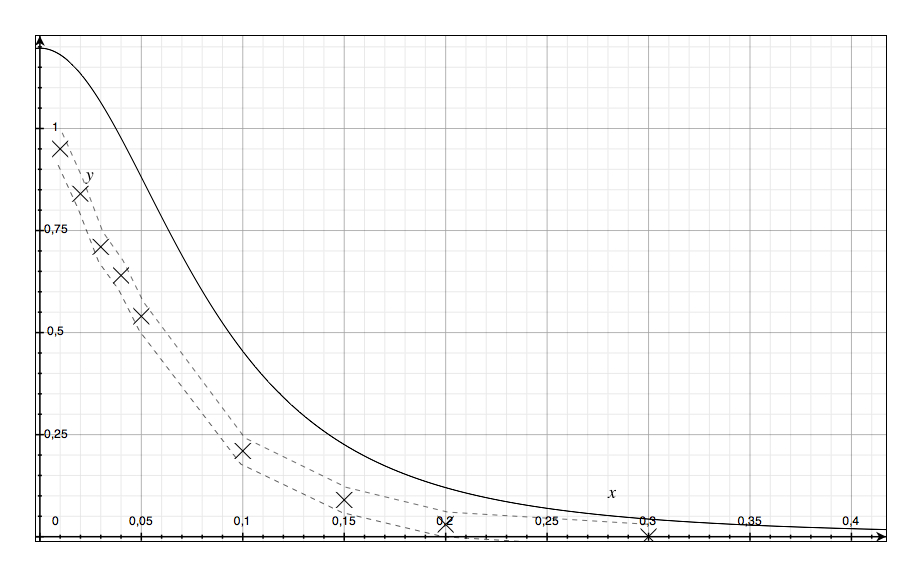
\includegraphics[scale=0.4]{labrapport-teoridel-ligning1.jpg}
\caption{Graf over målte verdier. Feilmarginer er angitt av stiplede grafer. Teoretisk ideell graf i blått i bakgrunn. }
\label{fig:maalteverdier}
\end{figure}


\begin{figure}[H]
\begin{center}
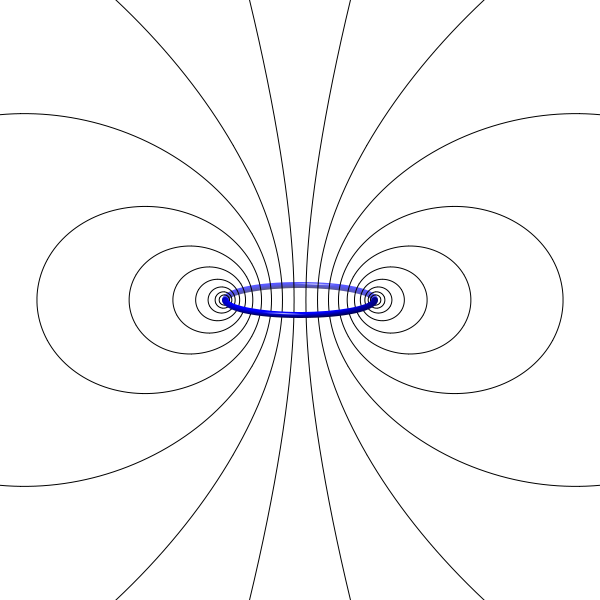
\includegraphics[scale=0.4]{magnetsime-rundt-spole.png}
\caption{Skisse over magnetfelt. Linjene viser hvordan magnetfeltet legger seg rundt spolen.}
\label{fig:skisse-magnetfelt}
\end{center}
\end{figure}



\clearpage


\subsection{Indusert spenning i spole}
Vi satte signalgeneratoren til sinusspenning, med en frekvens på 38,3 Hz.
Når vi så satte de små spolene inntill den store spolen, ble det indusert følgende spenninger i dem:\\
\begin{center}
$V_{400}$: $V_{pp}$ = 176 mV\\

$V_{2000}$: $V_{pp}$ = 900 mV\\
\end{center}
Signalet i begge de små spolene hadde en frekvens på 38,3 Hz, det samme som inngangssignalet.\\
\\
Observerer sammenhengen mellom indusert spenning og antall viklinger:\\

\begin{equation}
    \label{eq:viklinker1}
    \frac{2000 \textrm{ vikl.} }{400 \textrm{ vikl.} } = 5 \hspace{1.5cm} , \hspace{1.5cm} \frac{900 \textrm{ mV}}{176 \textrm{ mV}} = 5,11
\end{equation}\\
Vi skrudde så opp spenningen i generatoren, og målte nye verdier:\\
\begin{center}
$V_{400}$: $V_{pp}$ = 1880 mV\\

$V_{2000}$: $V_{pp}$ = 328 mV\\
\end{center}
Igjen er frekvensen 38.3 Hz. Vi sammenlikner verdier:\\

\begin{equation}
    \label{eq:viklinger2}
     \frac{2000 \textrm{ vikl.} }{400 \textrm{ vikl.} } = 5 \hspace{1.5cm} , \hspace{1.5cm} \frac{1800 \textrm{ mV}}{328 \textrm{ mV}} = 5,73
\end{equation}\\
Vi ser igjen at forholdet mellom antall viklinger og indusert spenning er (nesten) likt.

Vi konkluderer med at det er en lineær sammenheng mellom antall viklinger i de to spolene, og spenningen som blir indusert. Avviket tilskriver vi nok en gang motstand i spolene, samt at det var umulig å få spolene helt innpå hverandre, da det var en beskyttende plasthylse rundt.\\
\\
Vi observerer at spoler med forskjellig vikling kan brukes til å transformere en strøm fra en spenning til en annen, samtidig som man beholder frekvensen.

\clearpage
\subsection{Likestrømsmotor}
Her koblet vi opp motoren som anvist i figur 4.
Rotoren er laget slik at når den snurrer, vil strømretningen (og dermed magnetfeltet) snu seg ved hver halve omdreining.

De to statorene ble koblet slik at magnetfeltene sto "hver sin vei", dvs. at nordpolen var øverst på den ene siden, og nederst på den andre siden.
Rotorens nordpol vil frastøtes av statorens nordpol og tiltrekkes av statorens sydpol (og omvendt for rotorens sydpol).

 Når rotorens nordpol når fram til statorens sydpol ville den stoppet, om ikke konstruksjonen hadde vært slik at strømretningen internt i rotoren snudde. Siden strømen i rotoren snur, vil magnetfeltet rundt rotoren også snu, og polene er igjen frastøtende slik at rotoren fortsetter.


\begin{figure}[H]

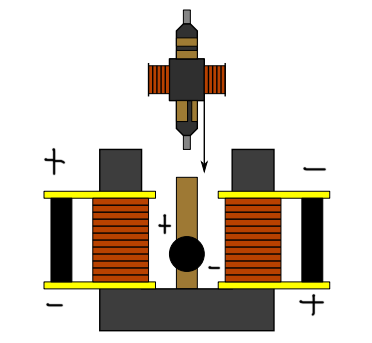
\includegraphics{motor.png}
\caption{Likestrømsmotor}
\label{fig:motor}
\end{figure}
\clearpage

\section{Konklusjon}
Vi har vist med relativt stor tydelighet at mengden indusert spenning fra én spole til en annen er lineært avhengig av antall viklinger i spolene, samt hvordan to spoler med forskjellig antall viklinger sammen fungerer som en transformator.\\
\\
Vi har også vist at teorien for magnetfelt rundt en spole oppfører seg som vist i ligning [\ref{eq:magnetfelt-spole}]. \\
\\
I tillegg har vi ved å konstruere en fungerende likestrømsmotor, vist at magnetisme har en reell praktisk applikasjon.
\clearpage

\section{Litteraturhenvisninger}
{[1]}Labheftet fra NTNU: alle likninger og teori, oppgavetekst:  \url{http://home.phys.ntnu.no/brukdef/undervisning/tfy4125_lab/oppgaver/oppgave4_tfy4125.pdf} \\
{[2]}Wolfram Alpha: Jordens magnetfelt i Trondheim: \url{http://www.wolframalpha.com/input/?i=magnetic+field+trondheim}


\end{document}







